\documentclass[conference]{IEEEtran}
\IEEEoverridecommandlockouts
% The preceding line is only needed to identify funding in the first footnote. If that is unneeded, please comment it out.
\usepackage{cite}
\usepackage{amsmath,amssymb,amsfonts}
\usepackage{algorithmic}
\usepackage{graphicx}
\usepackage{textcomp}
\usepackage{xcolor}
\pagecolor{white}
\def\BibTeX{{\rm B\kern-.05em{\sc i\kern-.025em b}\kern-.08em
    T\kern-.1667em\lower.7ex\hbox{E}\kern-.125emX}}
\graphicspath{ {./images/} }   
\begin{document}

\title{Enhancing Path Efficiency: Innovations in the Artificial Feeding Birds Algorithm for Solving TSP Problems\\
}

\author{\IEEEauthorblockN{1\textsuperscript{st} Given Name Surname}
\IEEEauthorblockA{\textit{dept. name of organization (of Aff.)} \\
\textit{name of organization (of Aff.)}\\
City, Country \\
email address or ORCID}
\and
\IEEEauthorblockN{2\textsuperscript{nd} Given Name Surname}
\IEEEauthorblockA{\textit{dept. name of organization (of Aff.)} \\
\textit{name of organization (of Aff.)}\\
City, Country \\
email address or ORCID}
}

\maketitle

\begin{abstract}
This document is a model and instructions for \LaTeX.
This and the IEEEtran.cls file define the components of your paper [title, text, heads, etc.]. *CRITICAL: Do Not Use Symbols, Special Characters, Footnotes, 
or Math in Paper Title or Abstract.
\end{abstract}

\begin{IEEEkeywords}
component, formatting, style, styling, insert
\end{IEEEkeywords}

\section{Introduction}

\input{./tsp.tex}
\section{Basic AFB Algorithm}
\section{Methodology}
We structure our experiments in an incremental manner.
Each improvement in section \ref{Improvements} builds on the previous adjustments,
even if it is not explicitly noted.
We verify our improvements using a set of selected TSP problems from TSPLIB, namely
eil101, pa561, pr1002, u2156 and pr2392, ranging from 101 to 2392 cities.

For each experiment, we run the problems 10 times each to account for the randomness
at initialization, to reduce noise, and make it statistically significant.
In order to then compare the performance of different experiments
we record the \textit{Mean Percentage Error}, over the 50 tests, with respect to the optimal solutions.
We also record the \textit{Mean Runtime} in seconds.

\begin{equation}
Percent Error= \frac{\lvert measured - optimal\rvert}{optimal}*100
\end{equation}

All experiments are executed on a MacBook Pro (M1 Pro) 2021.
\section{Improvements} \label{Improvements}
\subsection{Considerations about number of birds}
If we study the effects of how different number of birds change the solution of different tours, we learn that less birds seem to yield better solutions. At first this may seem counterintuitive, but there is an intuitive explanation to this:

The basic algorithm defines one iteration as the calculation for the cost of one tour. Now, let a phase of the algorithm denote each bird performing one move. So, in each phase each bird performs one move.
If we now use more birds the number of phases the algorithm will run through will decrease, as in each phase the length of more tours will be calculated, which will use up more iterations. Therefore, the more birds we have, the more iterations we will use up per phase, which means the algorithm will run through less phases until it stops. 
Because in one phase each bird can perform one move, less phases mean each bird can perform less moves. Less moves in turn leads to a less pronounced search of possible solutions, which will make the algorithm worse. This is why the less birds we have, the better the results will be.
Examples can be seen in Figure ... (fig about relationship n birds x cost).

One could avoid this by simply increasing the number of iterations, which balances the relationship between number of birds used and the results obtained. However, this inevitable leads to longer running times.

Consequently, we focus on improving the bird behavior, so that each bird needs fewer overall steps to achieve a good solution.
(say something about the number of iterations used in experiments and how this relates to the facts described above)
At the end of our analysis we will revisit this behavior and conduct if our improvements changed the relationship discussed above (Chapter \ref{Effect of improvemens on number of birds}).

\subsection{Swarm Behavior} \label{Swarm Behavior}
Currently, if one big bird made the decision to join another bird, he picks one randomly.
This means joining any bird without considering how good the position of that bird might be. This contradicts the original idea of the authors that big birds tend to join others that have found a good food source (current solution seems promising) \cite{afb}.
Therefore, we propose that a big will only be able to join the top-b percent of birds that have the lowest current cost. If one chooses the right ratio, we assume that it will automatically nudge the swarm in the direction of the global minimum.

We implement this by storing the indices $i$ of the birds in an ordered integer array $ord$ and introducing a new hyperparameter $b$, denoting which of the top-b percent to join. When we select the bird to join to, we draw a random uniform number $j$ between 1 and $b*n$ ($n$ denotes the number of birds) and get the index of the bird to join from the ordered array ($ord[j]$).

The main disadvantage this approach has is that at we need to continuously update $ord$ so that we only join the actual top-b percent at the moment of the move.
We decide to update the list after each bird has performed one move (after each phase).
This will still increase the computational complexity, but we think that this is better than updating the list after each move, as this would be too costly.

We test numerous values for $b$ and decide to build on $b=0.01$ for future improvement, as this strategy yields the best results (Table \ref{top_b_performance}). For intuitions on why such a low value performs this good, please refer to section \ref{Algorithm Stability}.

\begin{table}[h!]
\centering
\begin{tabular}{ |p{1.5cm}||p{0.75cm}|p{0.75cm}|p{0.75cm}|p{0.75cm}|p{0.75cm}|p{0.75cm}|p{0.75cm}|  }
 \hline
 Top-b& 1 & 0.25 & 0.20 & 0.15 & 0.05 & 0.01&\textbf{only best}\\
\hline \hline
 PercentError & 497 &323 & 279 &  246 & 150 & 79 &\textbf{69}\\
 \hline
 Time (in s) & \textbf{19.7} & 21.8 & 21.3 &  21.3 & 21.7 & 21.4 & 20.8\\
 \hline
\end{tabular}
\caption{Comparison of different parameters for our top-join. 1 means 100\%, so a bird randomly joins another bird. This is our benchmark and the
default behavior of the algorithm. Time is measured as the median runtime in seconds, over all tests.}
\label{top_b_performance}
\end{table}

\subsection{3-opt Walk}

For the walk move the algorithm uses a modified version of the 2-opt heuristic as a local search \cite{afb}. Instead of using 2-opt, we test a 3-opt variant, as this often yields the best solutions under consideration of computational complexity \cite{lin}. At the same time we decide to remove the estimation of local similarity from the algorithm, as the authors did not provide any intuitions why this may be beneficial \cite{afb}.

With 3-opt, each bird selects the tour with the lowest cost out of the 7 different tours possible.
At which 3 points a tour is opened is determined by a random uniform draw of 3 integers,
denoting the nodes of the tour. Because we now need to calculate the length of each of the possible 7 tours
in just one move, we decide it will still only cost us one iteration.
The results can be seen in Table \ref{3_opt_performance}.

\begin{figure}[htbp]
\centerline{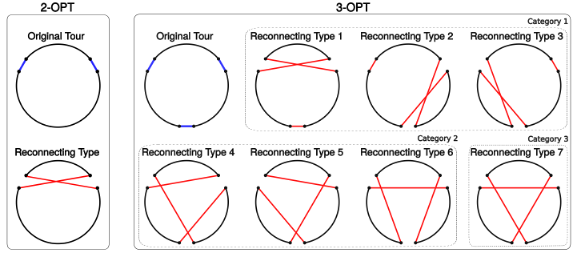
\includegraphics[width=8cm]{3_opt}}
\caption{Comparison of 2-opt (left) and 3-opt (right) for TSP. Reconnections of category 1 are 2-opt variants \cite{3_opt}.}
\label{3_opt}
\end{figure}

\begin{table}[h!]
\centering
\begin{tabular}{ |p{2cm}||p{0.75cm}|p{0.75cm}|  }
 \hline
 Configuration& 2-opt & \textbf{3-opt}\\
 \hline \hline
PercentError & 69 & \textbf{44}\\
 \hline
 Time (in s) & \textbf{21} & 85\\
 \hline
\end{tabular}
\caption{}
\label{3_opt_performance}
\end{table}

\subsection{Delegating Responsibility}

Because we are not implementing the 3-opt algorithm as an iterative solver by itself,
but rather in a swarm algorithm, in which each bird (or agent respectively) can perform this action,
the computational complexity will rise by a margin, as seen in Table \ref{3_opt_performance}.
In order to now compensate for this increase in complexity, we decide to test if we can delegate
the responsibility of performing 3-opt to only a subset of the birds. This sounds promising, as
we can reduce the computational complexity while still being able to profit from the increased exploration of 3-opt.

We test the case where only big birds are able to perform a 3-opt walk, while smaller birds
are only capable of the usual 2-opt walk as specified in the paper. 
This should not only reduce the computational complexity, but it also pairs well with the 
assumption that big birds are "superior", as only they can join other birds and therefore profit from them.

For the sake of completeness we also test the inverse approach: Only small birds can perform 3-opt.
Surprisingly, for big birds we observed that we can achieve the same performance as before, while
cutting runtime by half (Table \ref{3_opt_big_small_performance}). Interestingly, for small birds
we noticed an increased error rate, even though the small bird ratio is always $r > 0.5$ in our experiments.
Based on the results, we decided to use 3-opt only for big birds in our future experiments, as there
seems to be no downside to this approach.

\begin{table}[h!]
\centering
\begin{tabular}{ |p{2cm}||p{0.75cm}|p{0.75cm}|p{0.75cm}|p{0.75cm}|  }
 \hline
 Configuration& 2-opt & 3-opt & \textbf{3-opt big birds} & 3-opt small birds\\
 \hline \hline
PercentError & 69 & \textbf{44} & \textbf{44} & 85\\
 \hline
 Time (in s) & \textbf{21} & 85 & 40 & 69\\
 \hline
\end{tabular}
\caption{}
\label{3_opt_big_small_performance}
\end{table}

\subsection{Nearest-Neighbor Initialization}
\subsection{Early Stopping}
If we analyze the convergence behavior by plotting the cost of the best solution over the number of iterations
(Figure TODO),
we notice that our improved version of the algorithm converges much faster than the original algorithm,
even without a Nearest-Neighbor initialization. Because it is difficult to estimate how many iterations
are needed for a certain problem, and adapting the number of iterations to the problem at hand would
be cumbersome, we decide to implement an early stopping mechanism.
That way we do not waste computational resources on iterations that do not improve an existing solution,
which will reduce the runtime even further, especially for smaller TSP configurations, while retaining
a similar performance.

We implement this by introducing a new hyperparameter $p$, denoting the number of phases
without an improvement of the best current solution. If it is exceeded, the algorithm will stop.
This requires us to store the best solution over all birds and updating it continuously.
Fittingly, this is already implemented through the top-b join (see section \ref{Swarm Behavior}),
as we already need to store the best solution over all birds in order to determine which bird
to join to. This is also the reason why we only check if the best solution has improved after each phase,
and not after each iteration, as during a phase this solution is not updated.
A review during a phase therefore does not make sense.

\begin{table}[h!]
\centering
\begin{tabular}{ |p{2cm}||p{1.5cm}|p{0.75cm}|  }
    \hline
    Early Stopping& No (default) & Yes \\
    \hline \hline
    PercentError & \textbf{8} & 10\\
    \hline
    Time (in s) & 42 & 9\\
    \hline
\end{tabular}
\caption{}
\label{early_stopping_performance}
\end{table}
\section{Analysis}
\subsection{Metabirds}
\subsection{Intuitions on our Improvements} \label{Intuitions on our Improvements}
Swarm algorithm usually include action of agents which can either be classified as exploitation or exploration.
Exploitation means an agent uses its current result and tries to improve it, i.e. the agent continues to go into the direction he previously went in the search tree/space.
For AFB, this is can be achieved using the walk move, so a local search.

Exploration means an agent tries to find a better solution not necessarily dependent on its current solution,
as is the case with exploitation. Therefore, it can be seen as a global search. For AFB, this can be achieved using the fly move.


For a swarm algorithm to deliver a good approximation with respect to the global minimum
it needs a good balance between exploitation and exploration:
It needs to be able to improve a good solution,
and search for different solutions if the current one does not seem promising.

If exploitation is too dominant, then the algorithm might get stuck in a local minimum, as other solutions (for TSP other, vastly different tours) will not be explored enough, and vice versa.

As might have come apparent in the sections prior, the main focus of this paper
was on exploitation (improving a good solution).
This is mainly done by the introduction of 3-opt and that big birds can only join successful birds.
Even though the latter cannot be seen directly as a local search, is does lead to more (big) birds performing exploitation of the solutions of other birds.

We explicitly do not modify the fly move, i.e. selecting a random tour, as this provides us with a rich selection of other possible solution, which at the same time is completely independent of the current solution (of an agent).

The prior is crucial for the success of our algorithm, because the extreme join
behavior modeled by the algorithm has a high danger of getting it stuck in a
local minimum: Starting with our improvements on the swarm behavior,
a big bird will only be able to join the best bird. Because which bird is the best
is not updated within a phase, it could be that during one phase a lot of big birds join the same bird,
putting a lot (not all, as a join is a matter of probability) of agents at one place in the search space.
The fly move enables birds to escape this single solution if it does not seem promising.

Furthermore, there is only a limited number of big birds, meaning small birds are able
to explore the search space elsewhere, while the big birds are focusing on the currently best performing bird.

Therefore, we get an algorithm that has an empirically tested balance between exploitation and exploration.
It exploits good solutions in a harsh manner while also being able to switch to completely new solutions if they prove to be better.
This process will be repeated until a solution is reached that will either be close to the optimum, or a local minimum.
Either way, the algorithm converges.

\subsection{Exploitators and Explorators}
The base algorithm consists of two types of agents, small and big birds.
With our improvements it may have been noticeable that we separated the roles
of both agent types more and more from each other:
While small birds can perform the usual 2-opt local search when they are walking,
big birds can perform a more powerful 3-opt walk;
big birds can join other birds.
We do this in order to make the components contained in each swarm algorithm,
exploration and exploitation, a more explicit part of the algorithm:
We delegate small birds to the role of explorators, and big birds to the role of exploitators.

Small birds are able to access vastly different areas of the search space for possible better
solutions than their current one. Using the fly-move, big birds are able to profit
from those birds that have found the best current solution by joining them and
improving that solution using 3-opt (walk).


The circumstance that small birds can also perform exploitation, using their own version of the walk move,
is owed to the fact that they otherwise would only be able to perform
the fly move, i.e. jumping between random solutions.
This wouldn’t be a good foundation for the join behavior of big birds (see Table \ref{small_birds_only_fly}),
which is essential for the performance of our algorithm.
Also, since big birds can also join other big birds,
and the solutions for small birds would be rather poor, the probability that
big birds will exclusively join other big birds would be very high,
making small birds essentially useless.

Exactly this can be verified by simply by comparing how 
the algorithm performs when (1) small birds can only fly,
(2) all small birds are removed from the algorithm, and only big birds are kept.

Surprisingly, the results show us that configuration (2) performs even better
than the variant (1), indicating that the big birds only
join other big birds, and that small birds, whose only purpose is to perform the fly move,
provide no value to the algorithm.

\begin{table}[h!]
\centering
\begin{tabular}{ |p{1.5cm}||p{1.2cm}|p{1.2cm}|p{2cm}| }
 \hline
 Configuration& \textbf{Regular} & Only fly& No small birds\\
 \hline \hline
PercentError & \textbf{8} & 15 & 10\\
\hline
\end{tabular}
\caption{If small birds are only able to fly, the algorithm performs worse than before.
Notice however that it still achieves a reasonable performance.
For our experiments we continuously used 200 birds, 150 of them being small birds.
So by removing all small birds for experiment (2), we are left with 50 (big) birds.}
\label{small_birds_only_fly}
\end{table}

%\input{./sop.tex}


\section*{References}

\begin{thebibliography}{00}
\bibitem{lin} Lin, S. (1965), Computer Solutions of the Traveling Salesman Problem. Bell System Technical Journal, 44: 2245-2269. https://doi.org/10.1002/j.1538-7305.1965.tb04146.x
\bibitem{afb} Jean-Baptiste Lamy. Artificial Feeding Birds (AFB): a new metaheuristic inspired by the behavior of pigeons. Advances in nature-inspired computing and applications, 2019, 10.1007/978-3-319-96451- 5\_3 . hal-02264232
\bibitem{3_opt} Jingyan Sui, Shizhe Ding, Ruizhi Liu, Liming Xu, Dongbo Bu. Learning 3-opt heuristics for traveling salesman problem via deep reinforcement learning. Proceedings of The 13th Asian Conference on Machine Learning, PMLR 157:1301-1316, 2021.

\end{thebibliography}
\vspace{12pt}

\end{document}
